
\documentclass[11pt]{article}
\usepackage{../../Shared_Resources/Latex_Styles/General_Style} 
\usepackage{../../Shared_Resources/Latex_Styles/mcode} 

\usepackage[utf8]{inputenc}
\usepackage{hyperref}
\newcommand\bigO[1]{{\ensuremath{\mathcal{O}(#1)}}}
\newtheorem{theorem}{Theorem}
\usepackage{algorithm}
\usepackage{algpseudocode}
\algnewcommand\algorithmicinput{\textbf{Input:}}
\algnewcommand\algorithmicoutput{\textbf{Output:}}
\algnewcommand\Input{\item[\algorithmicinput]}%
\algnewcommand\Output{\item[\algorithmicoutput]}%

\usepackage{listings}

\lstset{ frame=single}

\begin{document}

\lstset{frameround=fttt,language=Matlab}

\lstMakeShortInline[columns=fixed]|

\makeheader{10 -- November 21, 2023}{Deterministic rank revealing factorizations for low rank approximation}

{\bf{Exercise 0 (Optional): Numerical stability of randomized Nystrom}} \\

Just as in last week's exercise, consider the MNIST data set and the matrix $A$ as defined in the project or in last week's exercise sheet (with a fixed value of $c$). \textbf{You'll have to be careful with this data set here and in your project because you have to make sure the data set is normalized, i.e. all the entries are between 0 and 1}. Take a relatively small sample of the training set. In this section you can use either last week's code or your code from your project. Consider two different types of sketching matrices, $\Omega_1, \Omega_2$. For different sketching dimensions of both types of matrices, compute the relative error of the low rank approximation in terms of the nuclear norm. Provide a graph that compares these errors. Comment on your findings. 


\bigskip

{\bf{Exercise 1: Tournament pivoting}} \\

The truncated SVD provides the best low rank approximation in terms of the Frobenius and L2 norms. Recall that the $QR$ decomposition with column pivoting relies on a permutation matrix $\Pi$ and computes the decomposition $A \Pi = QR$. There are many ways of building such permutation matrix. Let 

\begin{align*}
\rho_i(W) &= \frac{1}{\|W^{-1}[i, :]\| } \\
\chi_j(W) &= \|W[:, j]\|
\end{align*}

Consider the following theorem from \url{https://inria.hal.science/hal-02947991v2/document}:


\begin{theorem}
Let $A$ be an $m \times n$ matrix, $1 \leq k \leq \min(m, n)$. For any $f>1$ there exists a permutation matrix $\Pi$ such that the decomposition $A \Pi = QR$ verifies for all $(i, j) \in [1, k] \times [1, n-k]$, 

\[ (R_{11}^{-1}R_{12})_{ij}^2 + \rho_i^2(R_11)\chi_j^2(R_22) \leq f^2. \]

\end{theorem} 

Such factorization is called a strong RRQR factorization. \\

Recall tournament pivoting for deterministic column selection. (Refer to the image below).

\begin{enumerate}
   \item Consider a matrix $A$ partitioned into $4$ column blocks. Each processor has one of these blocks.
   \item Implement strong RRQR (there is a MATLAB implementation, you can use that as a template for building your own Python implementation). 
   \item For each block of columns, select $k$ columns using strong RRQR, save their indices are given in $I_{i0}$. Be careful with these indices, you might have to deal with "global" and "local" indices.
   \item In each processor output these indices $I_{00}, I_{10}, I_{20}, I_{30}$.
   \item Test your method with three different matrices: 
   \begin{itemize}
       \item $A = H_{n}DH_{n}^{\top}$, where $H_{n}$ is the normalized Hadamard matrix of dimension $n$, $D$ is a diagonal matrix of your choice. Pick $n$ to be "small".
       \item Load the normalized MNIST data set and build $A$ as in the project (or last week's exercises). Select a few columns and rows.
       \item Build $A$ from the MNIST data set with $2^{11}$ data points.
   \end{itemize}
   \item Comment your results with the different matrices. Do you notice a problem when you take more rows and columns using the MNIST data set?
   \item Using $I_{00}, I_{10}, I_{20}, I_{30}$ build a low rank approximation of $A$. Check the L2 norm of the error with respect to the error of the truncated SVD.
   \item Check if the singular values of these selected columns approximate well the singular values of $A$.
   \item Check if the diagonal elements of $R_{11}$ approximate well the singular values of $A$.
\end{enumerate}

\begin{figure}[H]
     \centering
     \begin{subfigure}[b]{0.5\textwidth}
         \centering
         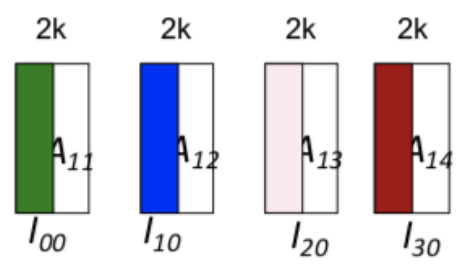
\includegraphics[width=\textwidth]{../figures/pivot.png}
     \end{subfigure}
\end{figure}

\end{document}
